\subsection{Performace Evaluation}

%\VT{ think in this section we can first qualitatively talk about potential performance
%issues, then briefly about simulation, then about performacnce evaluation results
%for pulls and pushes.}

While \sysname\ can significantly reduce the number of redundant files in the
Docker registry, it introduces overhead which can lead to potential performance
degradation.
%
The overhead can be split into two categories: 1)~\emph{background overhead} caused
by the additional computation and I/O that is performed during deduplicating and
restoring layers; and 2)~\emph{foreground overhead} which directly adds additional
processing on the critical path of a request.
%
%These above operations are either CPU intensive or I/O intensive, which would impact the
%foreground push/pull requests. The overhead of restoring a layer would become
%a bottleneck of a pull request.


\paragraph{Simulation}
%
\LR{We have to mention somewhere that we only considered layers smaller than 50\,MB.}
%
To analyze the impact of file-level deduplication, we conduct a preliminary simulation of
\sysname.
%
Based on the simulation result, we estimate the overhead of \sysname\ on
\texttt{push} and \texttt{pull} layer request latencies.
%
%We then provide different suggestions on how the Docker registry can mitigate
%the deduplication overhead.
%
%%%%%%%%%%%%%%%%%%%%%%%%%%%%%%%%%%%%%%%%%%%%%%%%%%%%%%%%%%%%%%%%%%%%%%%%%%%%
%
\begin{figure}
	\centering
	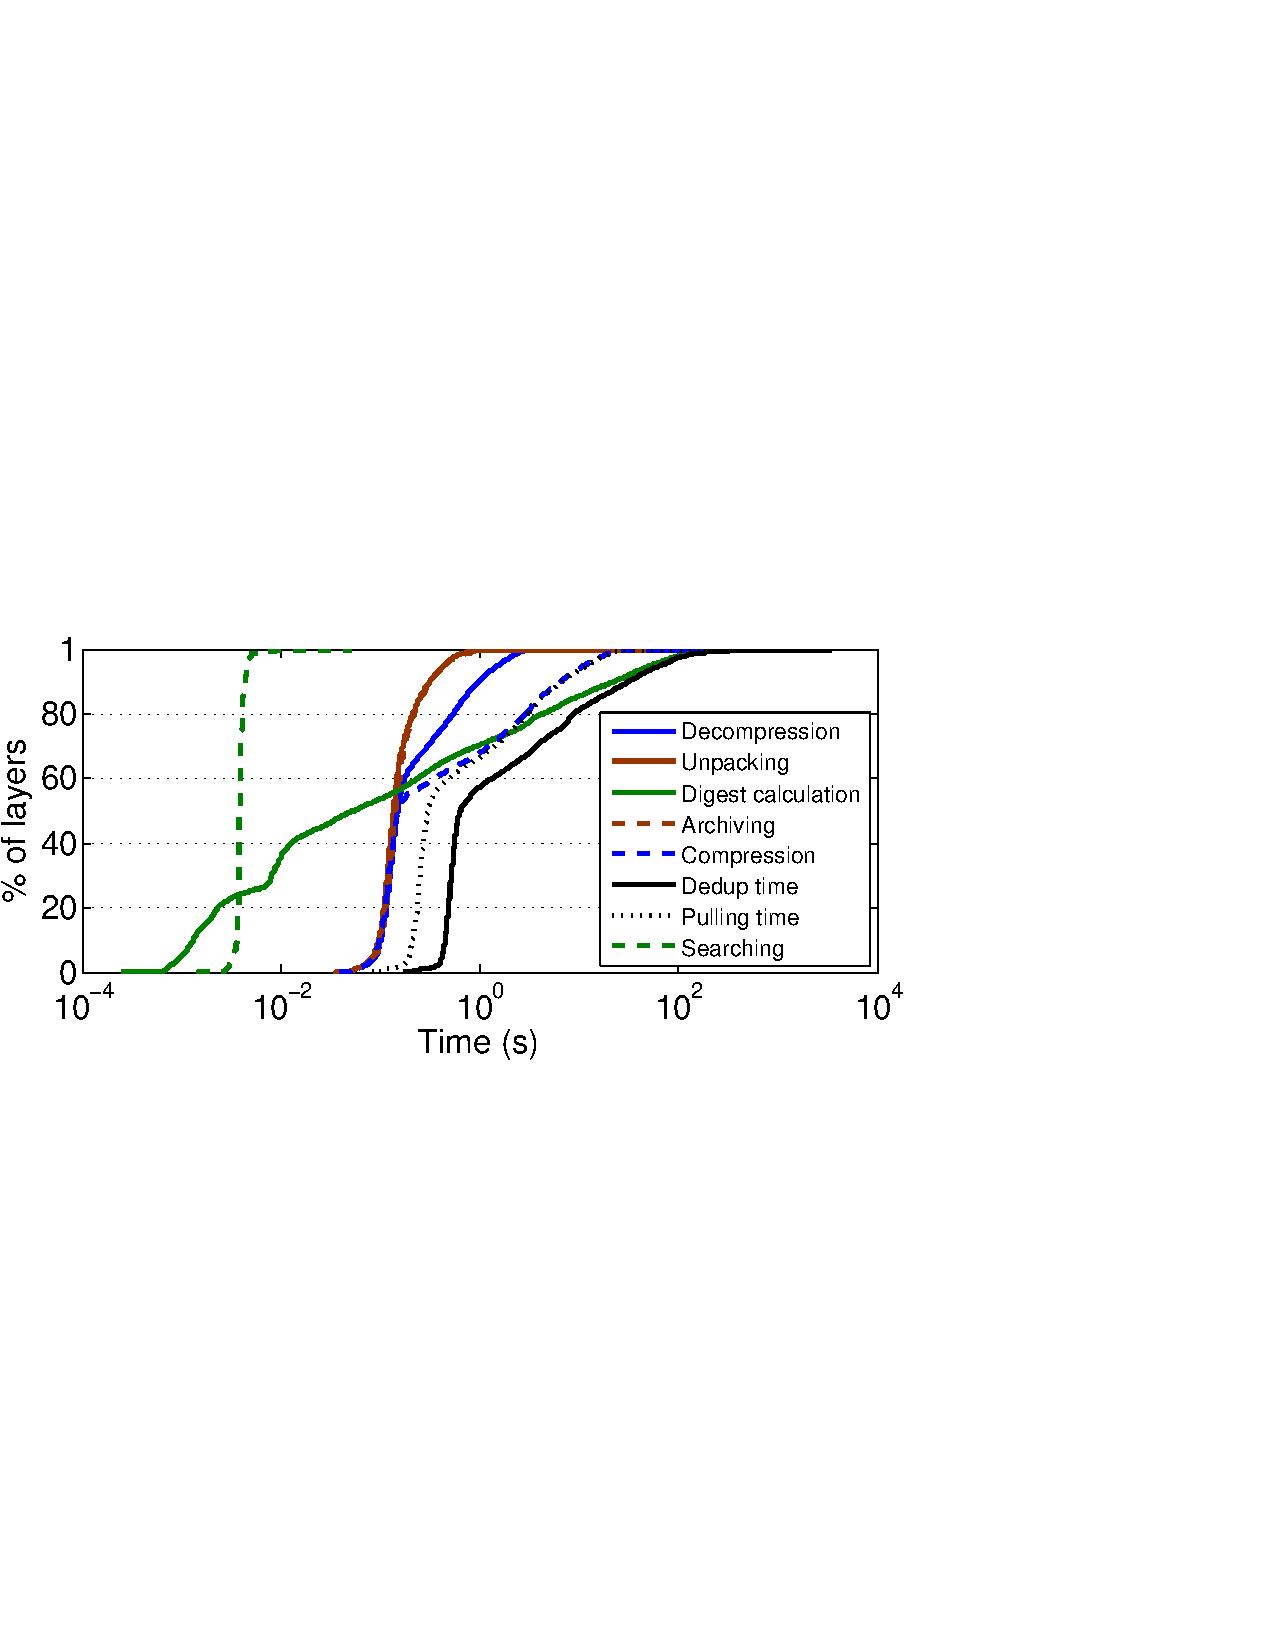
\includegraphics[width=0.5\textwidth]{graphs/res-time.pdf}
	\caption{Off-line file-level deduplication run time.}
	\label{fig:dedup-res}
\end{figure}

%
%\paragraph{Simulation} 
%
% since dedup process only starts periodically when the
%workload is lower and only cold layers are evolved in dedup process (discussed
%in Section~\ref{subsec:\sysname\}).
%
%\lrcomment{By latency, do you mean the time it takes to perform the dedup? I
%wouldn't call that latency but rather run time or completion time.}
%
%\lrcomment{What exactly was the setup? Where those 60 requests submitted while
%the dedup was running and where they submitted only once or repeatedly?}
%
%\LR{I think the flow in this subsection can be improved. Instead of the ``file-level deduplication
%	run time'' paragraph, I would introduce Fig~\ref{fig:dedup-res} at the end of the first paragraph,
%	right before ``Push layer latency'' and maybe explain the overal run time there. In the push and pull
%	layer latency we can then focus on just the parts of the graph that are related to push and pull.
%	This would be a more top-down presentation (which I feel often works better in papers).}
%\NZ{addressed}
%
%\LR{I'm still not sure if we should use simulation or emulation?}
%To study the overhead of file-level deduplication, we setup a
%one-node Docker registry with 64~GB RAM and 32 Cores.
%
%We then run file-level deduplication on the layer dataset.
%
%We then perform \emph{off-line} file-level deduplication
%operations on the layer dataset.
%

%\LR{We can remove the following steps once we explained them better
%	in 4.0}\NZ{addressed}
% 
%File-level deduplication mainly
%consists of the following steps: 
%layer decompression, 
%file content digest calculation,
%searching \& indexing,
%and storing unique files.
%The unique files are stored in a \textit{file pool}.

Our simulation follows the steps of \sysname\ as explained above:
First, a layer from the layer dataset is read and copied to a RAM disk. 
%
%Note that there is no foreground pull or push requests since the simulation is \emph{off-line}.
%
The layer is then decompressed and the fingerprints for each individual file
are computed by using the MD5 hash function~\cite{MD5}.
%
%\LR{How is the digest computed?}\NZ{addressed}
%
%\LR{\emph{emph} should be used instead of \textit{textit} to
%	emphasize certain words/parts in the text.}\NZ{addressed}
%
If the file has not been stored previously, we record the
file's fingerprint in a file index.
%
%And we append a \textit{layer-to-file} 
%mapping record to a mapping table. 
%
%\LR{This part is confusing. What does ``layer digest to its containing file content
%	digest mapping record'' mean? Why is it for each file in a layer and all layers?}
%\NZ{addressed}
%
To map a layer to its containing files, we create the layer recipe and add it
to a \emph{layer-to-file table}.
%
%For each file in a layer, a layer digest
%to its containing file content digest mapping record is also created 
%
%The \emph{layer-to-file table} also
%records the file path within each layer associated with each file.
%
Note that we do not consider the latency of storing unique files in our simulation.
%
After a layer has been deduplicated, it is again archived and compressed to
simulate a consequent \texttt{pull} request.
%
%Only unique files are maintained in RAM
%disk while the redundant copies are removed.
%

We implement the simulation in 600 lines of Python code
and set up a one-node Docker registry on a node with 32~cores and 64\,GB RAM.
%
We run \sysname\ for 0.9 million layers in total and process 60 layers in
parallel using 60 threads.
%
The overall runtime of the simulation was roughly 3.5 days.
%
%The overall runtime is about 3.5 days.

Figure~\ref{fig:dedup-res} shows the CDF for each sub-operation of
\sysname.
%
Unpacking, Decompression, Searching and Digest Calculation are part of
the deduplication process and together make up the Dedup time.
%
Archiving and Compression simulate the additional processing for a \texttt{pull}
request and form the Pulling time.
%
We see that 80\% of file-level deduplication time is less than 9.09\,s per layer
and our single-node deployment can process approximately 3 layers/s.
%
In a large-scale registry deployment, this throughput can be improved
as more node are available to perform deduplication.
%
%We suggest to use more high powerful machines to improve throughput.
%
Next, we look at the effects on \texttt{push} and \texttt{pull}
latencies in more detail.

%\LR{What was the overall runtime for processing 0.9 million layers?}\NZ{addressed}
%
%\alicomment{How are we saving the location
%of each file in the layer? It is not clear from the following sentences.}
%\NZ{addressed}
%
%To improve searching performance, the
%mapping table is stored in Hive database~\cite{xxx}. 
%
%\lrcomment{Why are we using Hive for this? It seems overkill to me, especially
%for such small data. Even at scale, a KeyValue store would probably provide
%better performance than clunky MapReduce-based DB.}
%

\paragraph{Push layer latency}

\sysname\ does not affect the latency of
\texttt{push} requests because deduplication is performed asynchronously, \ie
the registry reliably stores a copy of the layer as is and then sends a
response message to the user.
%
However, if there are intensive push requests while the registry is performing
deduplication, \sysname\ can still impact push latencies because it incurs CPU,
memory, and I/O overhead. %(similar to pull requests).

%Figure~\ref{fig:dedup-res} shows the breakdown of run time for each
%involved operation: decompression time, unpacking time, file content digest
%calculation time, and searching time.
%
Looking at the breakdown of the deduplication time in Figure~\ref{fig:dedup-res},
we make several observations:
%
\LR{Better to show the 90th percentile, that's a more commonly used value.}
\NZ{addressed}
First, we see that searching times are the smallest among all operations
and introduce negligible overhead with 90\% of search time being less than
0.004\,s. 
%
%The mapping table maintains 0.98 million layer-to-file digest mapping records. 
%
%\LR{Remove the following sentence? 1.7 million records is actually quite
%	small so even a single-node DB with one index is enough.}\NZ{addressed}
%Consider that more
%than 1.7 million layers are stored in Docker hub and the number is still
%increasing, it's better to choose a fast distributed database to provide high
%searching performance and scalability.
%
Second, we see that digest calculation times cover a wide range
from 0.000005\,s to 124.7\,s.
%
\LR{Shouldn't the distribution of those times then also be similar to the
layer size distribution?}
\NZ{it depends on layer size, file size, and the number of files}
This is because the time mainly depends on the layer size, \ie the fewer and smaller
files a layer contains, the faster it is to compute all digests for the layer.
%
%Typically, smaller layers contain a smaller number
%of smaller files, which takes much less time to calculate their digests.
%
%While if the layer is bigger, the digest calculation overhead will be higher. 
%
\LR{Again, better to show the 90th percentile.}
\NZ{90\% of digest calculation time is less than 27.1\,s.}
80\% of digest calculation time is less than 4.21\,s. 
%
%Thus, we suggest that multiple-threading is needed to calculate the files'
%digests simultaneously; 
%
%Fast CPUs as well as more powerful computing nodes are
%required to speed up digest calculation.
%
Third, the run time for decompression and unpacking follows the same distribution
for around 60\% of the layers and is less than 0.15\,s.
%
%Around 60\% of decompression and unpacking time are less than 0.15\,s. 
%
However, after that, the times diverge and compression times increase faster compared
to unpacking times.
%
\LR{Again, better to show the 90th percentile.}
\NZ{addressed}
90\% of decompression is less than 0.95 s while 90\% of packing time is less than 0.35\,s.

\LR{We need to draw some conclusions here.}
\NZ{Overall, we see that file digest calculation contributes a lot to the overall deduplication
latency especially when the layer size is big. 
Moreover, we see that the deduplication latency increases as the layer size grows.
}
\paragraph{Pull layer latency} 

For a \emph{pull layer} requests, \sysname\ will first fetch 
all its containing files by consulting the \emph{layer-to-file table}, 
restore the layer archive file and then send the compressed archive back
to the clients.

Figure~\ref{fig:dedup-res} shows the latency distributions for the compression
and archiving steps.
%
%Note that the \emph{pull layer} latency is the sum of archiving time,
%compression time, and searching time and does not include network transfer
%time.
%
%\LR{Always add a protected space or a \textbackslash, between a number and its unit.}
%\NZ{addressed}
%
We can see that around 55\% of the layers have a similar compression and archiving
time ranging from from 0.04\,s to 0.15\,s and both operations contribute equally
to pulling latency.
%60\% of compression and archiving time are less than 0.15 s.
%
%While compression has the highest run time 80\% of compression time is less than 2.82~s. 
%
\LR{Again, better to show the 90th percentile.}
\NZ{90\% of the compression time is less than 8\,s.}
After that, the times diverge and compression times increase faster with an
80\textsuperscript{ts} percentile of 2.82\,s.
%
Hence, compression time makes up the major portion of the pull latency and becomes a
bottleneck.
%
This is because compression times increase for larger layers and follow the distribution
of layer sizes (see Figure~\ref{fig:layer-size-cdf}).
%\LR{put reason here}
%\NZ{I think the layer size is the major reason}.
%
%We see that archiving time and compression contributes equally to pulling
%latency when their run time are lower than 0.15 s while compression time almost
%equals to pulling latency when the compression time is greater than 0.15 s. 

\LR{Should we move that to 4.3?}
%
\NZ{Can we use it as conclusion}
To reduce latency, we suggest that fast compression methods should be applied to reduce
compression times. As deduplication provides significant storage savings, faster compression
methods with a lower compression ratio are hence feasible.

%\alicomment{Separately mention pull layer requests}
%

%\paragraph{File-level deduplication run time}
